% Regression slice derived from the PGF manual's rectangle-split sizing rules.
% Horizontal splits ignore minimum width but keep minimum height.
\documentclass[tikz,border=2pt]{standalone}
\usetikzlibrary{shapes.multipart}
\begin{document}
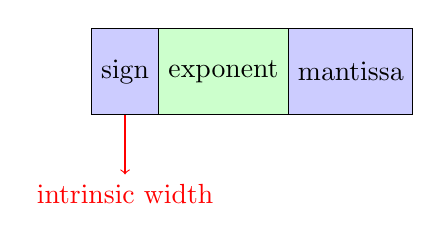
\begin{tikzpicture}
  \node[
    rectangle split,
    rectangle split horizontal,
    rectangle split parts=3,
    minimum width=8cm,
    minimum height=1.1cm,
    draw,
    rectangle split part fill={blue!20,green!20,blue!20}
  ] (parts) {sign\nodepart{two}exponent\nodepart{three}mantissa};
  \draw[red,->] (parts.one south) -- ++(0,-0.75cm) node[below] {intrinsic width};
\end{tikzpicture}
\end{document}
